% !TeX spellcheck = en_US

\chapter{Orbit correction}
\label{sec:correction}
\section{Some documented methods}

Several global corrections methods are well documented in the literature. The most common ones are the best corrector method and the response matrix method (see Sections~\ref{sec:most_effective_corr}) and \ref{sec:response_matrix}). 

Local orbit bumps (presented in Section~\ref{sec:orbit_bump}) allow local correction and are used to change the path of the orbit (during the injection time for example).

\subsection{Local orbit bumps}
\label{sec:orbit_bump}
\todo[inline]{see Wille p286}

\subsection{Most effective corrector method}
\label{sec:most_effective_corr}
This method is based on the fact that orbit shifts are often caused by strong localized disturbances. Its goal is to correct particularly each disturbance.

\subsubsection{Principle}

Given a distorted orbit, the optimal gain for each corrector is calculated by a mean square error algorithm (see \eqref{eq:gain_bestcorr}, \cite{book:wille}). The corrector which provides the best correction is selected: it is the most effective corrector.

Let's assume that the $i$th corrector, at position $s_i$, has the optical parameters $\beta_i$, $\alpha_i$ and $\Psi_i$, and that $m$ monitors are set around the orbit with parameters $\beta_j$, $\alpha_j$ and $\Psi_j$, and read a displacement $u_j$ from the reference orbit ($1 \leq j \leq m$).

The strength $\kappa_i$ of the field at the position $s_i$ is obtained minimizing the function
\todo{Explain in chap 1.3}
\begin{equation}
    \label{eq:gain_bestcorr}
    f_i(\kappa_i) = \sum\limits_{j=1}^{m} (u_j-x_{ij}(\kappa_i))^2 
                  = \sum\limits_{j=1}^{m} (u_j- \kappa_i h_{ij})^2
\end{equation}

with, if $\Delta \Psi_{ij} := \Psi_j-\Psi_i$,

\begin{align}
    \label{eq:hij}
    x_{ij}(\kappa_i) &= \kappa_i h_{ij} \nonumber\\
                     &= \kappa_i \frac{\sqrt{\beta_i \beta_j}}{2}
                         \left[
                             \frac{\cos(\Delta \Psi_{ij}) - 2\alpha_i \sin(\Delta\Psi_{ij})}
                                  {\tan (\pi Q)} + \sin (\Delta\Psi_{ij})
                         \right].
\end{align}

It follows that 
\begin{equation}
    \kappa_i = \frac{\sum\limits_{j=1}^m u_j h_{ij}}{\sum\limits_{j=1}^m h_{ij}^2}
\end{equation}

The $i$th corrector is attributed the gain $-\kappa_i$ to compensate the field.

\subsubsection{Iterative version}
When the most effective corrector is found, the process is reiterated on the corrected orbit with the remaining correctors. 

By doing this until all corrector are used (or that adding a correction does not improve the orbit) a comprehensive correction is reached.

\subsubsection{Practical issue}
The problem of this method is that each corrector must be tested once, and this for each iteration: the initialization of the correction is long and is then fixed.

Moreover, the correction is less efficient than the other ones presented here~\cite{book:wille}.

\subsection{Response matrix}
\label{sec:response_matrix}

This section is mainly based on~\cite{book:wille}, \cite{art:decker-1991} and \cite{art:plouviez-1999}.

The response matrix $\mat{S}$ is defined by the equation $\vec{X} = \mat{S}\, \vec{\Theta}$ where $\vec{\Theta}$ is the \emph{kick vector} and $\vec{X}$ the vector of \emph{orbit change}. If the accelerator has $M$ monitors and $N$ correctors, $\mat{S}$ is a $M \times N$ matrix.

Every coefficient $\mat{S}_{ij}$ is the orbit change at the position $s_i$ (of the $i$th monitor), for a kick of unity 1 at the position $s_j$ (of the $j$th corrector).

This matrix can be theoretically calculated by using the accelerator model and physics: $\mat{S}_{ij} = h_{ij}$ with the formula in \eqref{eq:hij}. However, the actual storage ring is never exactly the same as the designed one, because of several inaccuracies in its building. A more common way of constructing the response matrix is empirical: each measure cycle, a corrector is given a unitary value and the monitor are read, providing a column of the response matrix.

To do the correction, the inverse problem must be solved. We know the orbit change that we need to obtain a cleaner orbit, using the inverse of the response matrix will provide the correction to apply. Since it's very common to have more monitors than correctors, the matrix is not square. A \emph{singular value decomposition} (SVD) is used on the matrix to provide a pseudo-inversion.

Using the SVD also allows to use only the most significant singular values in the correction.\todo{why do we want this?}

\section{State of the art at BESSY II}

\subsection{The correction}
BESSY II currently uses a Fast Orbit Feedback (FOFB) which is based on a PID correction (proportional response with gain P, integral response with gain I and derivative response with gain D) and the response matrix inversion. The full process goes as presented in Fig.~\ref{fig:block_correction}.

\begin{figure}[!h]
    \centering
    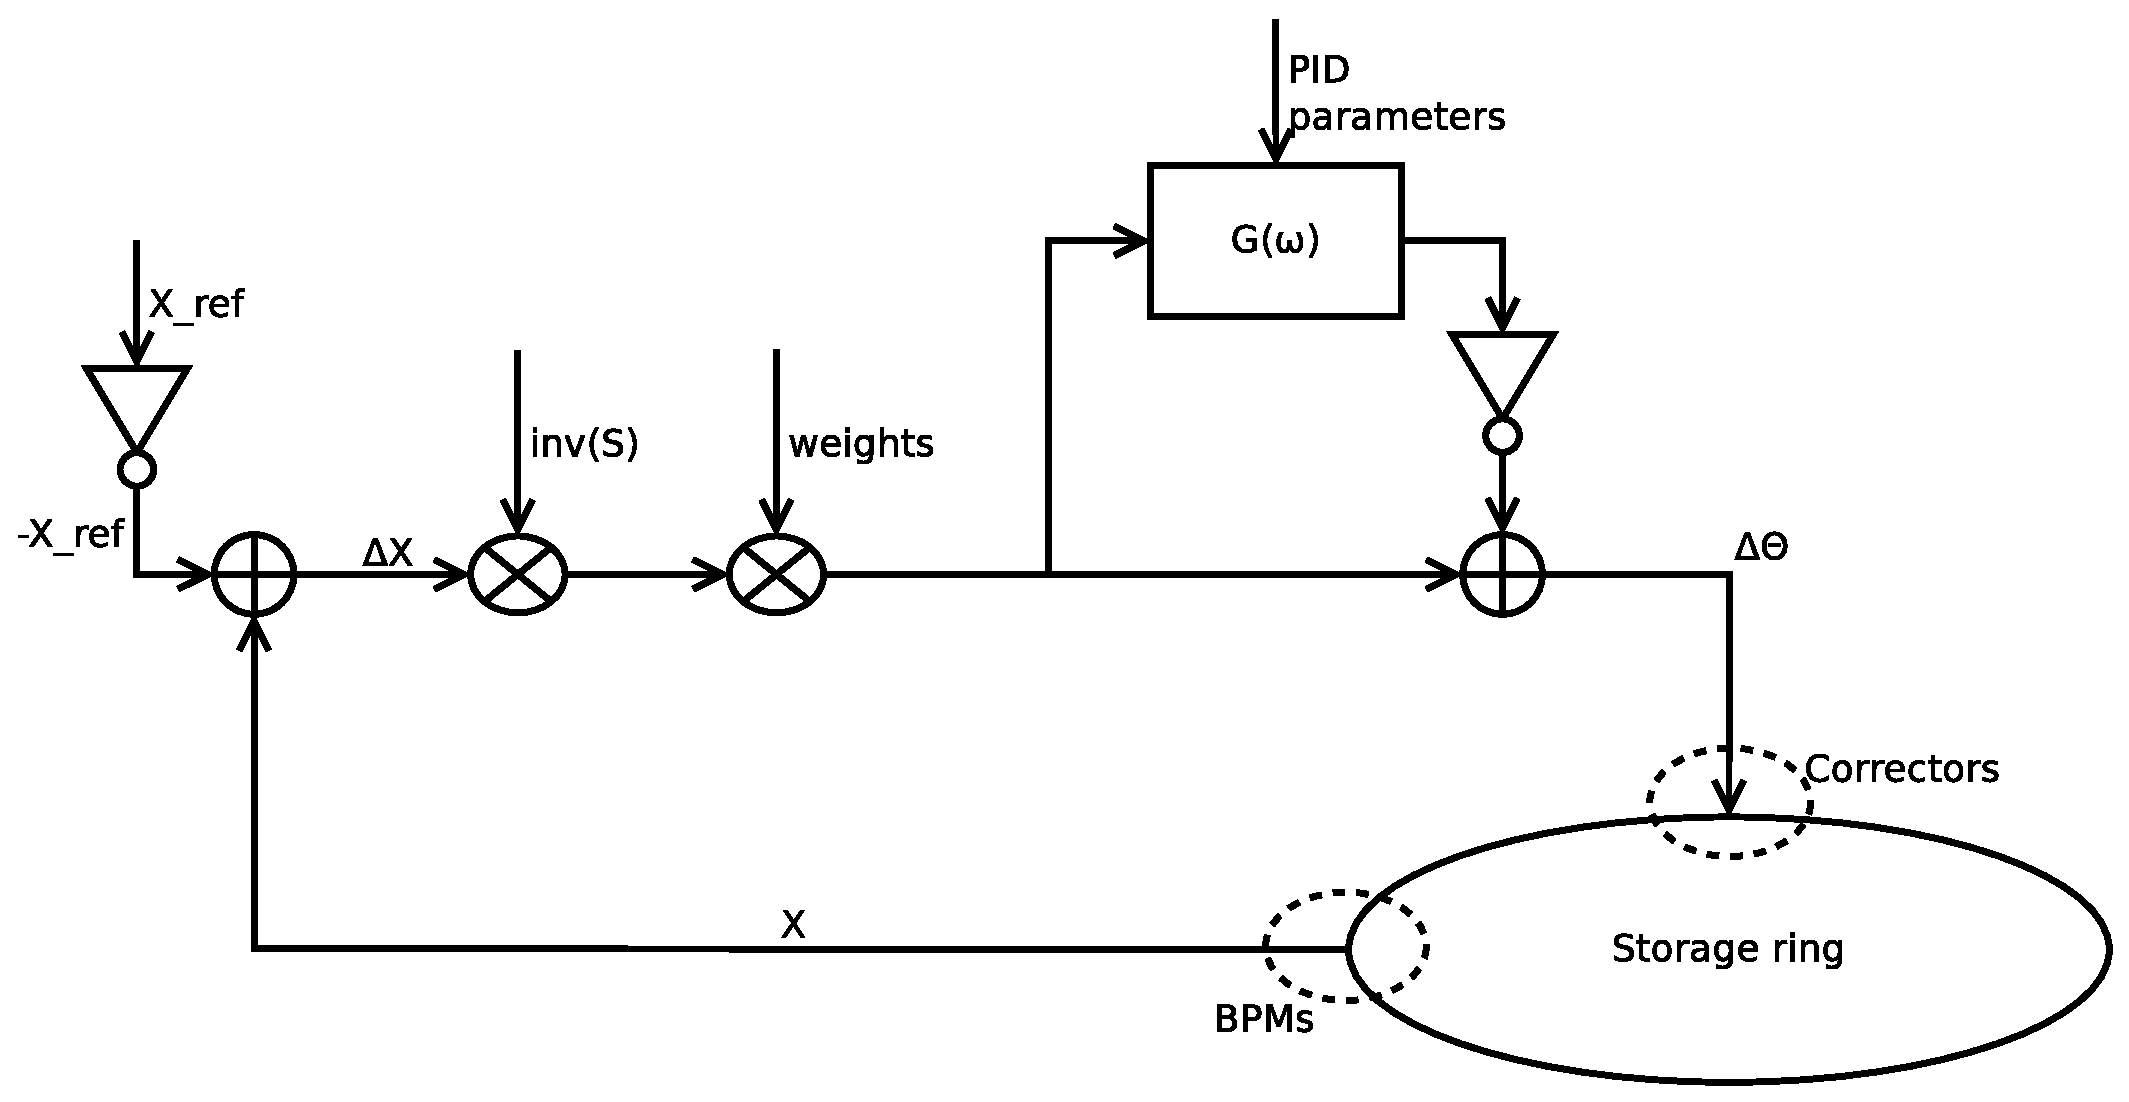
\includegraphics[width=.85\linewidth]{img/correction}
    \caption{\label{fig:block_correction}The correction process}
\end{figure}

\todo[inline]{Should I explain this here with words as well? \newline
    is it $\Delta \Theta$ or $\Theta$ (The real corrector value or the change to add)?\newline
    Why do we need this PID \textbf{\textit{exactly}}?}

\begin{align}
   & \Delta \vec{X} := \vec{X}-\vec{X}_\text{ref} \nonumber \\
   & \Delta \vec{\Theta}_t :=  \mat{S}^{-1} \Delta \vec{X} \odot \vec{W} \nonumber\\
   & G(\omega) = P + \frac{I}{\omega} + D \omega \qquad \text{(the PID)}\nonumber \\
   & \Delta \vec{\Theta} = \left[1-G(\omega)\right] (\Delta \vec{\Theta}_t)
\end{align}
with $\odot$ the point-wise multiplication and, $\vec{W}$ the vector of weights.

\remark The PID gains is not exactly as presented here: to prevent a too violent correction that might destabilize the current in the ring, the proportional gain is increased every correction round by 1\% until it reaches its nominal value.

\remark The PID is implemented as (for the $n$th correction round): 
\begin{equation*}
    P \times \Delta \vec{\Theta}_t(n) + I \times \sum\limits_{k=0}^{n-1}\Delta \vec{\Theta}_t(k) + D \times \left[\Delta \vec{\Theta}_t(n) - \Delta \vec{\Theta}_t(n-1)\right]
\end{equation*}

\subsection{Technical overview}

The correction is naturally automatized. Because the read/write actions should be really fast, a specific infrastructure was designed. This is represented on Fig.~\ref{fig:cbox_mbox}. 

\begin{figure}[!h]
    \centering
    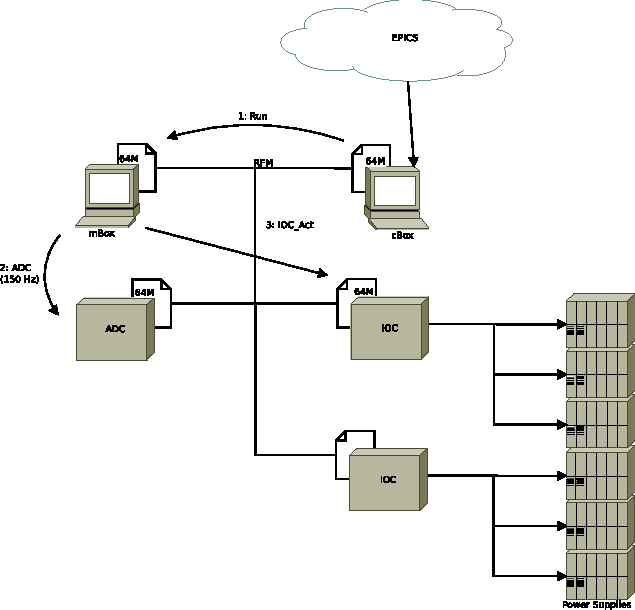
\includegraphics[width=.85\linewidth]{img/mBox_cBox}
    \caption{\label{fig:cbox_mbox}cBox and mBox: the correction infrastructure in BESSY II}
\end{figure}

All elements are connected to a reflective memory (RFM), which provides a high speed and low latency interface. This memory space is split in specified divisions to prevent data collisions.

Two main processes are operating:
\begin{itemize}
    \item the \textbf{cBox}. It controls (= \textit{c}) the correction. It defines when to read the values of the BPMs and when to write the new correction values, it provides initializations values. The operators are communicating with this process to configure the correction.
    \item the \textbf{mBox}. It does the math (= \textit{m}) of the correction. When allowed by the cBox, it reads the BPMs values, do the maths to define the new correction values and write them to the communication bus. This process also publish the values it reads and write so that client programs can subscribe to this data stream and reuse the values internally.
\end{itemize}

After having received the command to run from the cBox, the mBox queries the ADC (Analog-to-Digital Converter) to provide the BPM values in the RFM. The correction is then calculated (in Amperes) and the values are converted in a format easily transmissible. This data is written back to RFM and read by the IOCs (Input-Output Controllers) that relay to the power supplies alimenting the corrector magnets.

The full process is repeated at a frequency of 150~Hz. 

\section{Acquisition of the transfer matrix}
